\chapter{Weather Effects: Rain Fade \& Fog Attenuation}
\label{ch:weather-effects}

\begin{nontechnical}
\textbf{Think of radio waves like light beams traveling through the air.}

When it rains, you notice that:
\begin{itemize}
\item \textbf{Headlights look dimmer} through heavy rain
\item \textbf{You can't see as far} in fog
\item \textbf{Everything gets blurry} during a storm
\end{itemize}

\textbf{The exact same thing happens to satellite TV, 5G cell signals, and WiFi}---but you can't see it with your eyes.

\subsection*{The Core Problem}

\textbf{Raindrops absorb and scatter radio waves}, weakening the signal. The problem is worse when:

Raindrops absorb and scatter radio waves, weakening the signal. The problem is worse when:
\begin{enumerate}
\item \textbf{Higher frequencies} (like 5G's ``millimeter wave'') are used
  \begin{itemize}
  \item Think: FM radio (low frequency) works fine in rain, but satellite internet (high frequency) struggles
  \end{itemize}
\item \textbf{Heavier rain} falls
  \begin{itemize}
  \item Light drizzle: barely noticeable
  \item Thunderstorm: your satellite dish might lose connection entirely
  \end{itemize}
\item \textbf{Longer distances} through the weather
  \begin{itemize}
  \item Short WiFi connection (30 feet): rain doesn't matter much
  \item Satellite signal (22,000 miles up): crosses miles of rain clouds
  \end{itemize}
\end{enumerate}

\subsection*{Real-World Examples You've Experienced}

\textbf{Satellite TV going out during storms:}
\begin{itemize}
\item Your dish is trying to receive a signal from space
\item Heavy rain blocks 50--90\% of the signal strength
\item Below a threshold $\rightarrow$ ``Searching for signal\ldots''
\item This is called \textbf{rain fade}
\end{itemize}

\textbf{Slower 5G during rain:}
\begin{itemize}
\item 5G ``mmWave'' uses very high frequencies (like satellite dishes)
\item Rain weakens the signal between tower and your phone
\item Phone automatically switches to slower but more reliable 4G
\item You don't notice the rain, just ``slower internet''
\end{itemize}

\textbf{Why your GPS still works:}
\begin{itemize}
\item GPS uses lower frequencies (1.5~GHz) than satellite TV (12+~GHz)
\item Rain barely affects it (like how radio stations work in any weather)
\end{itemize}

\subsection*{The Math Part (Optional)}

The technical sections below answer questions like:
\begin{itemize}
\item \textbf{``Exactly how much weaker?''} (e.g., 10~dB loss = 90\% power lost)
\item \textbf{``At what frequency does rain start mattering?''} ($\sim$10~GHz threshold)
\item \textbf{``How do engineers design systems that work in rain?''} (Add backup power, use multiple frequencies, switch to lower data rates)
\end{itemize}

\textbf{You don't need to understand the equations} to grasp the main point:

\textit{Rain affects high-frequency radio signals a lot, low-frequency signals barely at all. Engineers compensate by adding extra power, using smarter antennas, or accepting slower speeds during storms.}
\end{nontechnical}

\section{Overview}

\textbf{Weather significantly impacts RF propagation}, especially at frequencies above 10~GHz. Rain, fog, snow, and clouds introduce \textbf{frequency-dependent attenuation} that must be accounted for in link budgets.

\begin{keyconcept}
\textbf{Attenuation increases with three key factors:}
\begin{enumerate}
\item \textbf{Frequency:} Higher frequencies = more attenuation (10--100~GHz most affected)
\item \textbf{Precipitation rate:} Heavier rain = more loss (quadratic scaling)
\item \textbf{Path length:} Longer distance through weather = more cumulative loss
\end{enumerate}

\textbf{Critical for:} Satellite communications (Ku/Ka/V-band), 5G mmWave (28/39~GHz), point-to-point microwave links.
\end{keyconcept}

\section{Mathematical Description}

\subsection{Rain Attenuation}

\subsubsection{Physical Mechanism}

\textbf{Raindrops act as lossy dielectric spheres}, introducing two primary loss mechanisms:

\begin{keyconcept}
Weather attenuation increases with three primary factors:
\begin{enumerate}
\item \textbf{Frequency}: Higher frequencies experience greater attenuation (proportional to $f^{2-3}$ in most cases)
\item \textbf{Precipitation rate}: Heavier rainfall or denser fog causes more signal loss
\item \textbf{Path length}: Longer propagation paths through weather accumulate greater total attenuation
\end{enumerate}
\end{keyconcept}

\textbf{Frequency dependence:}
\begin{itemize}
\item \textbf{$< 10$ GHz:} Rain effects negligible ($\lambda \gg$ raindrop size)
\item \textbf{10--100 GHz:} Strong attenuation ($\lambda \approx$ raindrop size, 1--5~mm)
\item \textbf{$> 100$ GHz:} Extreme attenuation (THz communications impossible in rain)
\end{itemize}

\subsubsection{ITU-R Rain Attenuation Model}

\textbf{Standard method:} ITU-R P.838 and P.618

The \textbf{specific attenuation} (loss per kilometer) is given by:
\begin{equation}
\gamma_R = k \cdot R^\alpha
\end{equation}
where:
\begin{itemize}
\item $\gamma_R$ = Specific attenuation (dB/km)
\item $R$ = Rain rate (mm/hr)
\item $k, \alpha$ = Frequency-dependent coefficients (from ITU tables)
\end{itemize}

The total path attenuation is:
\begin{equation}
A_{\text{rain}} = \gamma_R \times d_{\text{eff}}
\end{equation}
where:
\begin{itemize}
\item $A_{\text{rain}}$ = Total rain attenuation (dB)
\item $d_{\text{eff}}$ = Effective path length through rain (km)
\end{itemize}

\subsubsection{Rain Attenuation vs Frequency}

The following diagram shows how rain attenuation increases dramatically with frequency:

\begin{center}
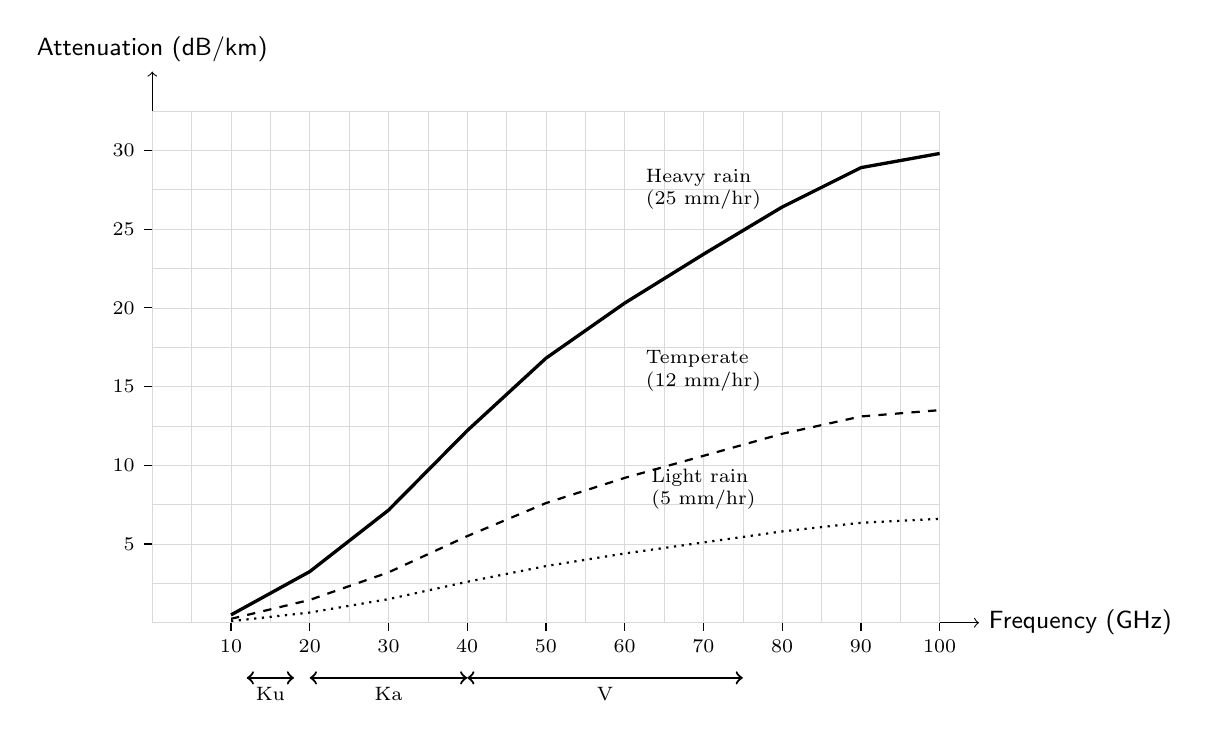
\begin{tikzpicture}[scale=1.0]
% Axes
\draw[->] (0,0) -- (10.5,0) node[right] {\sffamily\small Frequency (GHz)};
\draw[->] (0,0) -- (0,7) node[above] {\sffamily\small Attenuation (dB/km)};

% Grid
\draw[very thin,gray!30] (0,0) grid[step=0.5] (10,6.5);

% Frequency ticks
\foreach \x/\label in {1/10,2/20,3/30,4/40,5/50,6/60,7/70,8/80,9/90,10/100} {
  \draw (\x,0) -- (\x,-0.1) node[below,font=\scriptsize] {\label};
}

% Attenuation ticks
\foreach \y/\label in {1/5,2/10,3/15,4/20,5/25,6/30} {
  \draw (0,\y) -- (-0.1,\y) node[left,font=\scriptsize] {\label};
}

% Curve for 25 mm/hr rain (heavy rain)
\draw[very thick,black] 
  (1,0.1) -- (2,0.65) -- (3,1.43) -- (4,2.44) -- (5,3.36) -- 
  (6,4.06) -- (7,4.68) -- (8,5.28) -- (9,5.78) -- (10,5.96);

% Curve for 12 mm/hr rain (temperate)
\draw[thick,black,dashed] 
  (1,0.05) -- (2,0.29) -- (3,0.64) -- (4,1.1) -- (5,1.52) -- 
  (6,1.84) -- (7,2.12) -- (8,2.4) -- (9,2.62) -- (10,2.7);

% Curve for 5 mm/hr rain (light)
\draw[thick,black,dotted] 
  (1,0.02) -- (2,0.13) -- (3,0.3) -- (4,0.52) -- (5,0.72) -- 
  (6,0.88) -- (7,1.02) -- (8,1.16) -- (9,1.27) -- (10,1.32);

% Labels
\node[font=\scriptsize,align=left] at (7,5.5) {Heavy rain\\(25 mm/hr)};
\node[font=\scriptsize,align=left] at (7,3.2) {Temperate\\(12 mm/hr)};
\node[font=\scriptsize,align=left] at (7,1.7) {Light rain\\(5 mm/hr)};

% Band markers
\draw[<->,thick] (1.2,-0.7) -- (1.8,-0.7);
\node[below,font=\scriptsize] at (1.5,-0.7) {Ku};
\draw[<->,thick] (2,-0.7) -- (4,-0.7);
\node[below,font=\scriptsize] at (3,-0.7) {Ka};
\draw[<->,thick] (4,-0.7) -- (7.5,-0.7);
\node[below,font=\scriptsize] at (5.75,-0.7) {V};
\end{tikzpicture}
\end{center}

\paragraph{ITU Coefficients by Frequency}

\textbf{Selected values} (horizontal polarization):

{\def\LTcaptype{} % do not increment counter
\begin{longtable}[]{@{}llll@{}}
\toprule\noalign{}
Frequency & \(k\) & \(\alpha\) & Attenuation @ 25 mm/hr rain \\
\midrule\noalign{}
\endhead
\bottomrule\noalign{}
\endlastfoot
1 GHz & 0.0000387 & 0.912 & 0.0005 dB/km \\
4 GHz & 0.00065 & 1.121 & 0.025 dB/km \\
10 GHz & 0.0101 & 1.276 & 0.50 dB/km \\
12 GHz (Ku) & 0.0188 & 1.310 & 1.02 dB/km \\
20 GHz (Ka) & 0.0751 & 1.099 & 3.26 dB/km \\
30 GHz & 0.187 & 1.021 & 7.14 dB/km \\
40 GHz & 0.350 & 0.939 & 12.2 dB/km \\
50 GHz & 0.536 & 0.873 & 16.8 dB/km \\
60 GHz & 0.707 & 0.826 & 20.3 dB/km \\
80 GHz & 0.999 & 0.784 & 26.4 dB/km \\
100 GHz & 1.187 & 0.751 & 29.8 dB/km \\
\end{longtable}
}

\textbf{Note}: Vertical polarization has slightly different coefficients
(typically $\sim$10-20\% more attenuation)



\subsubsection{Rain Rate Classifications}

\textbf{ITU rain zones} (global climate regions):

{\def\LTcaptype{} % do not increment counter
\begin{longtable}[]{@{}
  >{\raggedright\arraybackslash}p{(\linewidth - 6\tabcolsep) * \real{0.0882}}
  >{\raggedright\arraybackslash}p{(\linewidth - 6\tabcolsep) * \real{0.1324}}
  >{\raggedright\arraybackslash}p{(\linewidth - 6\tabcolsep) * \real{0.5000}}
  >{\raggedright\arraybackslash}p{(\linewidth - 6\tabcolsep) * \real{0.2794}}@{}}
\toprule\noalign{}
\begin{minipage}[b]{\linewidth}\raggedright
Zone
\end{minipage} & \begin{minipage}[b]{\linewidth}\raggedright
Climate
\end{minipage} & \begin{minipage}[b]{\linewidth}\raggedright
Rain rate exceeded 0.01\% of year
\end{minipage} & \begin{minipage}[b]{\linewidth}\raggedright
Example locations
\end{minipage} \\
\midrule\noalign{}
\endhead
\bottomrule\noalign{}
\endlastfoot
A & Polar & 8 mm/hr & Arctic, Antarctic \\
B & Temperate & 12 mm/hr & Northern Europe, Canada \\
C & Subtropical & 22 mm/hr & Southern US, Mediterranean \\
D & Moderate tropical & 32 mm/hr & Southeast Asia, India \\
E & Equatorial & 42 mm/hr & Central Africa, Indonesia \\
F & Tropical maritime & 53 mm/hr & Amazon, Congo Basin \\
G & Monsoon & 63 mm/hr & Bangladesh, Myanmar \\
H & Intense tropical & 95 mm/hr & Extreme storms \\
\end{longtable}
}

\textbf{Design criterion}: Typically design for 99.9\% availability
(0.01\% outage time) - Temperate: 12 mm/hr - Tropical: 42-63 mm/hr



\section{Performance Analysis}

\subsection{Link Budget Impact: Satellite Examples}

\subsubsection{Example 1: Ku-Band Satellite (12~GHz Downlink)}

\textbf{Scenario:} GEO satellite $\rightarrow$ Home receiver, temperate climate

\textbf{Path geometry:}
\begin{itemize}
\item Elevation angle: $30°$
\item Slant path through rain: $\sim$6~km effective length
\item Rain rate (0.01\% time): 12~mm/hr
\end{itemize}

\textbf{Calculation:}

For Ku-band at 12~GHz with $k = 0.0188$ and $\alpha = 1.310$:
\begin{equation}
\gamma_R = k \cdot R^\alpha = 0.0188 \times 12^{1.310} = 0.50~\text{dB/km}
\end{equation}

Total path attenuation:
\begin{equation}
A_{\text{rain}} = \gamma_R \times d_{\text{eff}} = 0.50 \times 6 = 3.0~\text{dB}
\end{equation}

\textbf{Impact:} 3~dB margin needed for 99.9\% availability

\textbf{With 95~mm/hr extreme storm} (ITU zone H):
\begin{equation}
\gamma_R = 0.0188 \times 95^{1.310} = 6.3~\text{dB/km}
\end{equation}

\begin{equation}
A_{\text{rain}} = 6.3 \times 6 = 37.8~\text{dB}
\end{equation}

\begin{warningbox}
\textbf{Result:} Complete outage---attenuation exceeds typical 10--15~dB link margin. Satellite link becomes unusable during extreme storms without advanced mitigation techniques.
\end{warningbox}

\subsubsection{Example 2: Ka-Band Satellite (20~GHz Downlink)}

% Frequency markers
\draw[dashed,gray] (2,0) -- (2,-0.3) node[below,font=\scriptsize] {10};
\draw[dashed,gray] (8,0) -- (8,-0.3) node[below,font=\scriptsize] {100};

\textbf{Temperate climate (12~mm/hr):}

For Ka-band at 20~GHz with $k = 0.0751$ and $\alpha = 1.099$:
\begin{equation}
\gamma_R = 0.0751 \times 12^{1.099} = 1.16~\text{dB/km}
\end{equation}

\begin{equation}
A_{\text{rain}} = 1.16 \times 6 = 7.0~\text{dB}
\end{equation}

\textbf{Tropical climate (42~mm/hr):}
\begin{equation}
\gamma_R = 0.0751 \times 42^{1.099} = 4.4~\text{dB/km}
\end{equation}

\begin{equation}
A_{\text{rain}} = 4.4 \times 6 = 26.4~\text{dB}
\end{equation}

\begin{calloutbox}{Ka-Band Challenge}
\textbf{Comparison:} Ka-band suffers \textbf{2--3$\times$ more rain fade} than Ku-band!

\textbf{Mitigation strategies:}
\begin{itemize}
\item Adaptive coding/modulation (ACM) $\rightarrow$ Lower data rate in rain
\item Site diversity $\rightarrow$ Multiple ground stations (rain cells are localized)
\item Higher TX power margin (15--25~dB for tropical regions)
\end{itemize}
\end{calloutbox}

\subsubsection{Example 3: V-Band Satellite (40~GHz)}

\textbf{Next-gen satellite comms} (e.g., OneWeb, Starlink inter-satellite links):

\textbf{Temperate climate (12~mm/hr):}

For V-band at 40~GHz with $k = 0.350$ and $\alpha = 0.939$:
\begin{equation}
\gamma_R = 0.350 \times 12^{0.939} = 3.6~\text{dB/km}
\end{equation}

\begin{equation}
A_{\text{rain}} = 3.6 \times 6 = 21.6~\text{dB}
\end{equation}

\textbf{Result:} \textbf{Severe rain fade}---requires 25+~dB margin or advanced mitigation techniques such as site diversity and adaptive modulation.

\subsection{Terrestrial Path: 5G mmWave}

\subsubsection{Example 4: 28~GHz 5G Link (Urban Microcell)}

\textbf{Scenario:} Base station $\rightarrow$ UE, 200~m range, light rain (5~mm/hr)

\textbf{Calculation:}

For 28~GHz with $k = 0.187$ and $\alpha = 1.021$:
\begin{equation}
\gamma_R = 0.187 \times 5^{1.021} = 0.98~\text{dB/km}
\end{equation}

Path length $d = 0.2$~km:
\begin{equation}
A_{\text{rain}} = 0.98 \times 0.2 = 0.20~\text{dB}
\end{equation}

\textbf{Impact:} Minimal (short path length)

\textbf{Heavy rain (25~mm/hr):}
\begin{equation}
\gamma_R = 0.187 \times 25^{1.021} = 5.2~\text{dB/km}
\end{equation}

\begin{equation}
A_{\text{rain}} = 5.2 \times 0.2 = 1.0~\text{dB}
\end{equation}

\textbf{Conclusion:} 5G mmWave is \textbf{relatively rain-tolerant for short ranges} ($< 500$~m).

\subsubsection{Example 5: 60~GHz Point-to-Point Link}

\textbf{Scenario:} Building-to-building backhaul, 1~km, moderate rain (15~mm/hr)

\textbf{Calculation:}

For 60~GHz with $k = 0.707$ and $\alpha = 0.826$:
\begin{equation}
\gamma_R = 0.707 \times 15^{0.826} = 6.4~\text{dB/km}
\end{equation}

\begin{equation}
A_{\text{rain}} = 6.4 \times 1 = 6.4~\text{dB}
\end{equation}

\textbf{Plus oxygen absorption:} $\sim$15~dB/km at 60~GHz (clear air)
\begin{equation}
A_{\text{total}} = 15 + 6.4 = 21.4~\text{dB}
\end{equation}

\textbf{Result:} \textbf{60~GHz is impractical for $>1$~km in rain} (used for indoor/short-range only).

\section{Fog \& Cloud Attenuation}

\textbf{Fog = suspended water droplets} (smaller than rain, $\sim$10--100~$\mu$m diameter)

\textbf{Attenuation mechanism:} Primarily absorption (droplets $\ll \lambda$ for most RF bands)

\subsection{Fog Attenuation Model}

The \textbf{specific attenuation} due to fog is:
\begin{equation}
\gamma_{\text{fog}} = K_l \cdot M \quad \text{(dB/km)}
\end{equation}
where:
\begin{itemize}
\item $M$ = Liquid water content (g/m$^3$)
\item $K_l$ = Frequency-dependent coefficient
\end{itemize}

\textbf{Typical fog:}
\begin{itemize}
\item Light fog: $M = 0.05$~g/m$^3$
\item Dense fog: $M = 0.5$~g/m$^3$
\end{itemize}

\subsubsection{Coefficients by Frequency}

\subsection{Fog Attenuation Coefficients}

Table~\ref{tab:fog-coeffs} provides frequency-dependent fog attenuation coefficients.

\begin{table}[h!]
\centering
\caption{Fog attenuation coefficients and representative values}
\label{tab:fog-coeffs}
\begin{tabular}{@{}crr@{}}
\toprule
Frequency & $K_l$ (dB/km per g/m$^3$) & $\gamma$ (dense fog, $M = 0.5$~g/m$^3$) \\
\midrule
10~GHz & 0.01 & 0.005~dB/km \\
20~GHz & 0.07 & 0.035~dB/km \\
30~GHz & 0.20 & 0.10~dB/km \\
60~GHz & 1.0 & 0.50~dB/km \\
100~GHz & 2.5 & 1.25~dB/km \\
300~GHz & 15 & 7.5~dB/km \\
\bottomrule
\end{tabular}
\end{table}

\begin{keyconcept}
\textbf{Fog vs Rain:} Below 30~GHz, fog attenuation is \textbf{negligible compared to rain}. However, at terahertz frequencies ($>$ 100~GHz), fog becomes a significant impairment, particularly for short-range THz communication systems.
\end{keyconcept}

\subsection{Rain vs Fog: Comparative Analysis}

\subsubsection{Microwave/mmWave Regime (30~GHz, 1~km path)}

\begin{table}[h!]
\centering
\caption{Weather attenuation comparison at 30~GHz}
\label{tab:rain-fog-30ghz}
\begin{tabular}{@{}lr@{}}
\toprule
Weather Condition & Total Attenuation \\
\midrule
Clear air & $\sim$0.1~dB \\
Dense fog ($M = 0.5$~g/m$^3$) & 0.10~dB \\
Light rain ($R = 5$~mm/hr) & 3.7~dB \\
Moderate rain ($R = 12$~mm/hr) & 7.1~dB \\
Heavy rain ($R = 25$~mm/hr) & 12.5~dB \\
\bottomrule
\end{tabular}
\end{table}

\textbf{Conclusion:} At microwave and millimeter-wave frequencies, \textbf{rain dominates} weather-induced attenuation. Fog is negligible by comparison.

\subsubsection{Terahertz Regime (300~GHz, 100~m path)}

\begin{table}[h!]
\centering
\caption{Weather attenuation comparison at 300~GHz (THz)}
\label{tab:rain-fog-300ghz}
\begin{tabular}{@{}lr@{}}
\toprule
Weather Condition & Total Attenuation \\
\midrule
Clear air (water vapor) & $\sim$5~dB \\
Dense fog ($M = 0.5$~g/m$^3$) & 0.75~dB \\
Light rain ($R = 5$~mm/hr) & $>$ 300~dB (complete blockage) \\
\bottomrule
\end{tabular}
\end{table}

\begin{center}
\begin{tikzpicture}[scale=1.0]
% Title
\node[font=\sffamily\bfseries] at (5,5.5) {Attenuation vs Frequency: Rain vs Fog};

% Axes
\draw[->] (0,0) -- (10,0) node[right,font=\small] {Frequency (GHz)};
\draw[->] (0,0) -- (0,5) node[above,font=\small] {Attenuation (dB/km)};

% Grid
\draw[very thin,gray!30] (0,0) grid[step=1] (9,4.5);

% Rain curves (25 mm/hr)
\draw[thick,red,dashed] plot[smooth,tension=0.7] coordinates {
  (0.5,0.1) (1,0.2) (2,0.5) (3,1.0) (4,1.8) (5,2.8) (6,4.0) (7,5.5) (8,7.0) (9,8.5)
};
\node[right,font=\scriptsize,red] at (9.2,8.5) {Rain (25~mm/hr)};

% Fog curve (dense fog, 0.5 g/m³)
\draw[thick,blue] plot[smooth,tension=0.8] coordinates {
  (0.5,0.005) (1,0.01) (2,0.02) (3,0.04) (4,0.08) (5,0.15) (6,0.25) (7,0.40) (8,0.60) (9,0.85)
};
\node[right,font=\scriptsize,blue] at (9.2,0.85) {Fog (dense)};

% Frequency markers
\foreach \x/\label in {1/10, 3/30, 6/60, 9/90} {
  \draw[dashed,gray] (\x,0) -- (\x,-0.2) node[below,font=\scriptsize] {\label};
}

\textbf{Key insight}: Fog is \textbf{negligible below 30~GHz}, but significant at THz frequencies.

\subsection{Comparison: Rain vs Fog}

\begin{center}
\begin{tikzpicture}[scale=1.0]
% Axes
\draw[->] (0,0) -- (9,0) node[right] {\sffamily\small Frequency (GHz)};
\draw[->] (0,0) -- (0,7) node[above] {\sffamily\small Attenuation (dB/km)};

% Grid
\draw[very thin,gray!30] (0,0) grid[step=0.5] (8.5,6.5);

% Frequency ticks
\foreach \x/\label in {1/20,2/40,3/60,4/80,5/100,6/150,7/200,8/300} {
  \draw (\x,0) -- (\x,-0.1) node[below,font=\scriptsize] {\label};
}

% Attenuation ticks  
\foreach \y/\label in {1/2,2/4,3/6,4/8,5/10,6/12} {
  \draw (0,\y) -- (-0.1,\y) node[left,font=\scriptsize] {\label};
}

% Heavy rain (25 mm/hr)
\draw[very thick,black] 
  (1,0.65) -- (2,2.44) -- (3,4.06) -- (4,5.28) -- (5,5.96);

% Moderate rain (12 mm/hr)
\draw[thick,black,dashed] 
  (1,0.29) -- (2,1.1) -- (3,1.84) -- (4,2.4) -- (5,2.7);

% Dense fog (0.5 g/m³)
\draw[thick,black,dotted] 
  (1,0.07) -- (2,0.35) -- (3,1) -- (4,2) -- (5,2.5) -- (6,3.75) -- (7,5) -- (8,6);

% Labels
\node[font=\scriptsize,align=left] at (3.5,5.8) {Heavy rain\\(25 mm/hr)};
\node[font=\scriptsize,align=left] at (3.5,3.5) {Moderate rain\\(12 mm/hr)};
\node[font=\scriptsize,align=right] at (6.5,4.5) {Dense fog\\(0.5 g/m$^3$)};

% Annotation
\node[font=\scriptsize,align=center] at (1.5,6) {Rain\\dominates};
\node[font=\scriptsize,align=center] at (6.5,6) {Fog becomes\\significant};
\end{tikzpicture}
\end{center}

\textbf{At 30 GHz, 1 km path}:

{\def\LTcaptype{} % do not increment counter
\begin{longtable}[]{@{}ll@{}}
\toprule\noalign{}
Condition & Attenuation \\
\midrule\noalign{}
\endhead
\bottomrule\noalign{}
\endlastfoot
Clear air & $\sim$0.1 dB \\
Dense fog (0.5 g/m\textbackslash textsuperscript\{3\}) & 0.10 dB \\
Light rain (5 mm/hr) & 3.7 dB \\
Moderate rain (12 mm/hr) & 7.1 dB \\
Heavy rain (25 mm/hr) & 12.5 dB \\
\end{longtable}
}

\textbf{Rain dominates} at microwave/mmWave frequencies.

\textbf{Fog becomes important} at THz ($>$ 100 GHz):

\end{tikzpicture}
\end{center}

{\def\LTcaptype{} % do not increment counter
\begin{longtable}[]{@{}ll@{}}
\toprule\noalign{}
Condition & Attenuation \\
\midrule\noalign{}
\endhead
\bottomrule\noalign{}
\endlastfoot
Clear air & $\sim$5 dB (water vapor) \\
Dense fog & 0.75 dB \\
Light rain (5 mm/hr) & \textbf{300+ dB} (complete blockage) \\
\end{longtable}
}



\section{Snow \& Ice Attenuation}

\textbf{Dry snow:} Very low attenuation (air + ice crystals, low loss)
\begin{equation}
\gamma_{\text{dry snow}} \approx 0.0005 \times f^2 \times S \quad \text{(dB/km)}
\end{equation}
where:
\begin{itemize}
\item $f$ = Frequency (GHz)
\item $S$ = Snowfall rate (mm/hr liquid equivalent)
\end{itemize}

\textbf{Example:} At 20~GHz, 10~mm/hr dry snow:
\begin{equation}
\gamma \approx 0.0005 \times 20^2 \times 10 = 0.2~\text{dB/km (negligible)}
\end{equation}

\textbf{Wet snow} (melting): Much higher attenuation (comparable to rain)

\textbf{Ice crystals} (cirrus clouds): Minimal attenuation ($< 0.1$~dB even at 100~GHz)

\textbf{Practical implication:} Snow is \textbf{far less problematic} than rain for RF links.

\subsection{Hail Attenuation}

Different frequency bands exhibit vastly different susceptibility to rain attenuation, influencing their suitability for various applications.

\begin{table}[h!]
\centering
\caption{Rain sensitivity by frequency band}
\label{tab:band-sensitivity}
\begin{tabular}{@{}llll@{}}
\toprule
Band & Frequency & Primary Use & Rain Sensitivity @ 25~mm/hr \\
\midrule
C-band & 4--8~GHz & Satellite TV, radar & \textbf{Low} (0.05~dB/km) \\
X-band & 8--12~GHz & Military, radar & \textbf{Moderate} (0.5~dB/km) \\
Ku-band & 12--18~GHz & Satellite TV/broadband & \textbf{Moderate-High} (1--2~dB/km) \\
Ka-band & 26.5--40~GHz & Satellite, 5G backhaul & \textbf{High} (3--12~dB/km) \\
V-band & 40--75~GHz & Next-gen satellite & \textbf{Very High} (12--20~dB/km) \\
W-band & 75--110~GHz & Automotive radar & \textbf{Extreme} (20--30~dB/km) \\
\bottomrule
\end{tabular}
\end{table}

\textbf{C-band Advantage:} Widely deployed in tropical regions due to excellent rain tolerance. Lower bandwidth but highly reliable.

\textbf{Ka-band Challenge:} Offers high data rates and bandwidth, but requires adaptive coding/modulation (ACM) and large link margins (10--15~dB) to maintain availability.

\section{Mitigation Techniques}

Engineers employ several strategies to maintain link availability despite weather-induced attenuation.

\subsection{Static Link Margin}

The simplest approach is to \textbf{add extra power margin} to the link budget:

\begin{itemize}
\item Temperate climate, Ku-band: +3--5~dB
\item Tropical climate, Ka-band: +8--15~dB
\item mmWave terrestrial ($< 1$~km): +2--3~dB
\end{itemize}

\textbf{Trade-off:} Requires higher transmit power or larger antennas, increasing cost and complexity.

\subsection{Adaptive Coding and Modulation (ACM)}

ACM systems \textbf{dynamically adjust modulation order and coding rate} based on real-time link quality:

\begin{center}
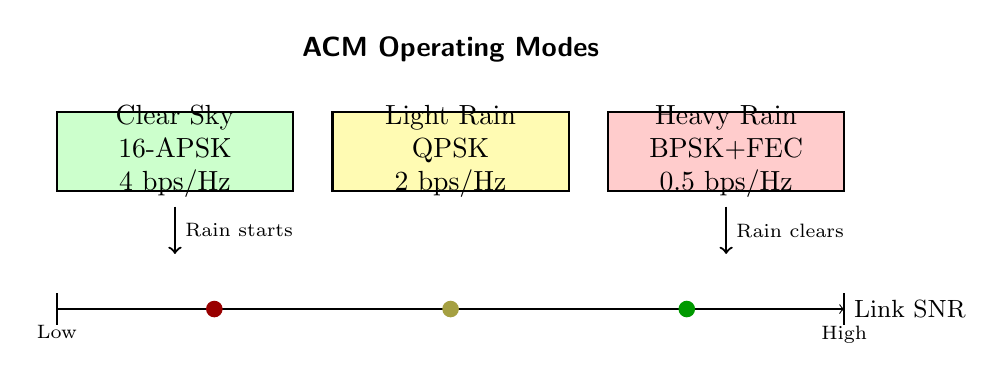
\begin{tikzpicture}[scale=1.0]
% Title
\node[font=\sffamily\bfseries] at (5,4.8) {ACM Operating Modes};

% States
\draw[fill=green!20,thick] (0,3) rectangle (3,4) node[pos=0.5,align=center] {Clear Sky\\16-APSK\\4 bps/Hz};
\draw[fill=yellow!30,thick] (3.5,3) rectangle (6.5,4) node[pos=0.5,align=center] {Light Rain\\QPSK\\2 bps/Hz};
\draw[fill=red!20,thick] (7,3) rectangle (10,4) node[pos=0.5,align=center] {Heavy Rain\\BPSK+FEC\\0.5 bps/Hz};

% Arrows showing transitions
\draw[->,thick] (1.5,2.8) -- (1.5,2.2) node[midway,right,font=\scriptsize] {Rain starts};
\draw[->,thick] (8.5,2.8) -- (8.5,2.2) node[midway,right,font=\scriptsize] {Rain clears};

% SNR axis
\draw[->] (0,1.5) -- (10,1.5) node[right,font=\small] {Link SNR};
\draw[thick] (0,1.3) -- (0,1.7) node[below=8pt,font=\scriptsize] {Low};
\draw[thick] (10,1.3) -- (10,1.7) node[below=8pt,font=\scriptsize] {High};

% Operating points
\fill[green!60!black] (8,1.5) circle (3pt);
\fill[yellow!60!black] (5,1.5) circle (3pt);
\fill[red!60!black] (2,1.5) circle (3pt);

\end{tikzpicture}
\end{center}

\textbf{Result:} Graceful degradation---system maintains connectivity at reduced data rate rather than complete outage.

\textbf{Applications:} DVB-S2 (satellite TV), 5G NR, VSAT modems.

\subsection{Site Diversity}

Multiple ground stations separated by 5--20~km exploit the \textbf{localized nature of rain cells} (typically 5--10~km diameter):

\begin{equation}
P_{\text{both fade}} = P_{\text{site 1}} \times P_{\text{site 2}} \times \rho
\end{equation}
where $\rho < 1$ is the spatial correlation factor.

\textbf{Diversity gain:} 5--10~dB improvement in link availability.

\textbf{Example:} Commercial satellite gateways deploy 2--3 geographically separated sites to achieve 99.99\% uptime.

\subsection{Uplink Power Control (UPC)}

UPC systems \textbf{increase transmit power during rain} to compensate for attenuation:

\begin{enumerate}
\item Monitor satellite beacon signal strength
\item Detect fade depth in real-time
\item Boost uplink power (typically up to 10~dB)
\item Avoid saturating satellite transponder
\end{enumerate}

\textbf{Limitation:} Power amplifier headroom is finite. Cannot compensate for extreme fades ($> 15$~dB).

\subsection{Orbit Selection}

Low Earth Orbit (LEO) satellites offer \textbf{inherently shorter rain paths}:

\begin{itemize}
\item \textbf{GEO} (36,000~km altitude): Rain path $\approx 6$~km at 30° elevation
\item \textbf{LEO} (550~km altitude): Rain path $\approx 2$~km at 30° elevation
\end{itemize}

\textbf{Result:} LEO systems experience approximately \textbf{3$\times$ less rain attenuation} than GEO for the same frequency and rain rate. This is a key advantage of Starlink and OneWeb constellations.

\section{Depolarization Effects}

Beyond simple attenuation, rain also causes \textbf{cross-polarization interference} due to the oblate (flattened) shape of raindrops.

\subsection{Physical Mechanism}

Raindrops are not spherical---they flatten into oblate spheroids as they fall. This asymmetry causes:
\begin{itemize}
\tightlist
\item
  Monitor beacon signal from satellite
\item
  Detect fade, boost uplink power (up to $\sim$10 dB)
\item
  Avoid saturating satellite transponder
\end{itemize}

\textbf{Limitation}: Power amplifier headroom (can't boost infinitely)



\subsubsection{6. Orbit Selection}

\textbf{Low Earth Orbit (LEO)} satellites have shorter slant paths:

The rain-induced XPD degradation is modeled by:
\begin{equation}
\text{XPD}_{\text{rain}} = U - V \log_{10}(A_{\text{rain}}) \quad \text{(dB)}
\label{eq:xpd-rain}
\end{equation}
where:
\begin{itemize}
\tightlist
\item
  GEO: $\sim$40,000 km, slant path through rain
  $\sim$6 km @ 30\$\^{}\textbackslash circ\$ elevation
\item
  LEO: $\sim$550 km, slant path $\sim$2 km @
  30\$\^{}\textbackslash circ\$ elevation
\end{itemize}

\textbf{Rain attenuation}:
\textbf{$\sim$3\$\textbackslash times\$ less for LEO} (shorter
path)

\textbf{Starlink/OneWeb advantage}: Better rain performance than GEO

\section{Worked Example: Ka-Band Link Budget with Rain Fade}

\textbf{Problem:} Design a Ka-band satellite link for 99.9\% availability in a tropical climate. Determine required link margin.

\subsection*{Given Parameters}

\begin{tabular}{@{}ll@{}}
Frequency & $f = 20$~GHz (Ka-band downlink) \\
Satellite altitude & GEO ($36{,}000$~km) \\
Elevation angle & $30°$ \\
Climate zone & Tropical (ITU zone E) \\
Rain rate (0.01\% time) & $R = 42$~mm/hr \\
TX power & $P_t = 100$~W = 50~dBm \\
TX antenna gain & $G_t = 35$~dBi \\
RX antenna gain & $G_r = 42$~dBi (1.5~m dish) \\
System noise temp & $T_s = 200$~K \\
Data rate & $R_b = 10$~Mbps \\
Required BER & $10^{-6}$ (requires $E_b/N_0 = 10.5$~dB) \\
\end{tabular}

\subsection*{Step 1: Calculate Effective Rain Path Length}

For $30°$ elevation angle:
\begin{equation}
d_{\text{eff}} = \frac{h_{\text{rain}}}{\sin(30°)} = \frac{4~\text{km}}{0.5} = 8~\text{km}
\end{equation}
where $h_{\text{rain}} = 4$~km is typical rain height in tropics.

\subsection*{Step 2: Calculate Rain Attenuation}

For 20~GHz, $k = 0.0751$, $\alpha = 1.099$:
\begin{equation}
\gamma_R = k \cdot R^\alpha = 0.0751 \times 42^{1.099} = 4.4~\text{dB/km}
\end{equation}

Total rain attenuation:
\begin{equation}
A_{\text{rain}} = \gamma_R \times d_{\text{eff}} = 4.4 \times 8 = 35.2~\text{dB}
\end{equation}

\subsection*{Step 3: Free-Space Path Loss}

\begin{equation}
\text{FSPL} = 20\log_{10}(36{,}000) + 20\log_{10}(20{,}000) + 32.45 = 211.0~\text{dB}
\end{equation}

\subsection*{Step 4: Clear-Sky Link Budget}

Received power (clear sky):
\begin{equation}
P_r = P_t + G_t + G_r - \text{FSPL} = 50 + 35 + 42 - 211 = -84~\text{dBm}
\end{equation}

Noise power ($B = 10$~MHz):
\begin{equation}
N = 10\log_{10}(kT_sB) = 10\log_{10}(1.38 \times 10^{-23} \times 200 \times 10^7) = -104~\text{dBm}
\end{equation}

SNR:
\begin{equation}
\text{SNR} = P_r - N = -84 - (-104) = 20~\text{dB}
\end{equation}

$E_b/N_0$:
\begin{equation}
\frac{E_b}{N_0} = \text{SNR} + 10\log_{10}\left(\frac{B}{R_b}\right) = 20 + 10\log_{10}(1) = 20~\text{dB}
\end{equation}

\subsection*{Step 5: Rainy Conditions}

Received power (rain):
\begin{equation}
P_r = -84 - 35.2 = -119.2~\text{dBm}
\end{equation}

New $E_b/N_0$:
\begin{equation}
\frac{E_b}{N_0} = 20 - 35.2 = -15.2~\text{dB}
\end{equation}

\subsection*{Step 6: Required Link Margin}

\begin{equation}
\text{Margin required} = A_{\text{rain}} + \text{Implementation loss} = 35.2 + 3 = 38.2~\text{dB}
\end{equation}

\begin{calloutbox}[colback=black!8!white,colframe=black]{Link Budget Summary}
\textbf{Answer:} The link requires a \textbf{38~dB margin} for 99.9\% availability in tropical conditions.

\textbf{Interpretation:}
\begin{itemize}
\item Clear sky: $E_b/N_0 = 20$~dB (9.5~dB margin)
\item During 42~mm/hr rain: Link \textbf{fails} without mitigation
\item Required: Implement ACM to reduce data rate during rain, OR use site diversity, OR add 38~dB more TX power (impractical)
\end{itemize}

\textbf{Solution:} Deploy ACM that can drop to BPSK + FEC, reducing effective data rate to 2~Mbps during heavy rain, providing 7~dB coding gain and recovering the link.
\end{calloutbox}

\section{Depolarization Effects}

\textbf{Rain also causes cross-polarization:}

\textbf{Mechanism:} Raindrops are \textbf{oblate} (flattened spheres)
\begin{itemize}
\item Horizontal and vertical polarizations experience different phase shifts
\item Converts co-pol energy $\rightarrow$ cross-pol
\end{itemize}

\textbf{Impact:} Degrades dual-polarization systems (e.g., V/H reuse for 2$\times$ capacity)

\subsection{Cross-Polarization Discrimination (XPD)}

The XPD degradation due to rain is given by:
\begin{equation}
\text{XPD}_{\text{rain}} = U - V \log(A_{\text{rain}}) \quad \text{(dB)}
\end{equation}
where:
\begin{itemize}
\item $U, V$ = Frequency-dependent constants ($\sim$30--40~dB, $\sim$12--20~dB typical)
\item $A_{\text{rain}}$ = Co-pol attenuation (dB)
\end{itemize}

\textbf{Example:} If rain causes 10~dB attenuation:
\begin{equation}
\text{XPD}_{\text{rain}} = 30 - 12\log(10) = 30 - 12 = 18~\text{dB}
\end{equation}

XPD degrades from 30~dB (clear) to $\sim$18~dB, reducing dual-pol isolation.

\subsection{Regional Considerations}

\subsubsection{Temperate Climates (Europe, Northern US, Canada)}

\textbf{Rain characteristics:}
\begin{itemize}
\item Moderate intensity (12--22~mm/hr, 0.01\% time)
\item Long-duration stratiform rain (hours)
\item Lower fade durations
\end{itemize}

\textbf{Design approach:}
\begin{itemize}
\item Standard margins (3--5~dB for Ku, 8--12~dB for Ka)
\item ACM effective (gradual fade)
\end{itemize}

\subsubsection{Tropical Climates (Southeast Asia, Equatorial Africa, Amazon)}

\textbf{Rain characteristics:}
\begin{itemize}
\item High intensity (42--95~mm/hr, 0.01\% time)
\item Short-duration convective storms (minutes)
\item High fade depths
\end{itemize}

\textbf{Design approach:}
\begin{itemize}
\item Large margins (8--15~dB for Ku, 15--25~dB for Ka)
\item Site diversity essential for Ka-band
\item C-band preferred for critical services
\end{itemize}

\textbf{Case study:} Indonesia (equatorial)
\begin{itemize}
\item Ku-band outages: $\sim$0.5\% of time (annual)
\item Ka-band: $\sim$2--5\% (unacceptable without mitigation)
\item C-band: $< 0.01\%$ (reliable)
\end{itemize}

\section{Measurement \& Prediction}

\subsection{Radiometer Method}

\textbf{Measure sky brightness temperature} $T_B$:
\begin{equation}
A_{\text{rain}} = 10 \log\left(\frac{T_{\text{sky}} - T_B}{T_{\text{sky}} - T_{\text{medium}}}\right) \quad \text{(dB)}
\end{equation}
where:
\begin{itemize}
\item $T_B$ = Measured brightness temperature (K)
\item $T_{\text{sky}}$ = Clear sky temperature (K)
\item $T_{\text{medium}}$ = Physical temperature of rain medium (K)
\end{itemize}

\textbf{Real-time fade monitoring} for UPC systems.

\subsubsection{Weather Radar Integration}

\subsection{Design Guidelines}

\begin{enumerate}
\item \textbf{Frequency Selection:}
  \begin{itemize}
  \item C-band: Robust in all climates, bandwidth-limited
  \item Ku-band: Good balance for temperate regions
  \item Ka-band: High capacity, requires mitigation
  \item mmWave: Only for short terrestrial or inter-satellite links
  \end{itemize}

\textbf{Proactive ACM}: Adjust modulation before fade hits (minimize disruption)

\section{Applications}

\subsection{Satellite Communications}

\textbf{GEO Ku-band (12--18~GHz):}
\begin{itemize}
\item Direct-to-home TV (DirecTV, Dish Network)
\item VSAT broadband
\item Typical margins: 3--8~dB (temperate), 8--15~dB (tropical)
\item Rain fade mitigation: ACM, site diversity for gateways
\end{itemize}

\textbf{GEO Ka-band (20--30~GHz):}
\begin{itemize}
\item High-throughput satellites (HTS)
\item Viasat, HughesNet broadband
\item Higher capacity but rain-sensitive
\item Required: Advanced ACM, large margins (15--25~dB tropical)
\end{itemize}

\textbf{LEO Constellations (Ku/Ka):}
\begin{itemize}
\item Starlink, OneWeb, Kuiper
\item Shorter path through rain ($\sim$2--3~km vs 6--8~km for GEO)
\item Better rain performance (2--3$\times$ less attenuation)
\item Enables reliable Ka-band service
\end{itemize}

\subsection{5G mmWave}

\textbf{28/39~GHz bands:}
\begin{itemize}
\item Urban microcells ($<$ 500~m range)
\item Rain impact: 0.5--2~dB typical
\item Acceptable for short ranges
\item Beam steering compensates for fading
\end{itemize}

\textbf{Design consideration:} Network densification provides inherent diversity (multiple base stations available).

\subsection{Point-to-Point Microwave}

\textbf{E-band (71--86~GHz):}
\begin{itemize}
\item Cellular backhaul
\item Range limited to $<$ 1~km in rain
\item Requires backup link (lower frequency)
\item Regulation-free spectrum advantage
\end{itemize}

\subsection{Mitigation Strategies Comparison}

\begin{center}
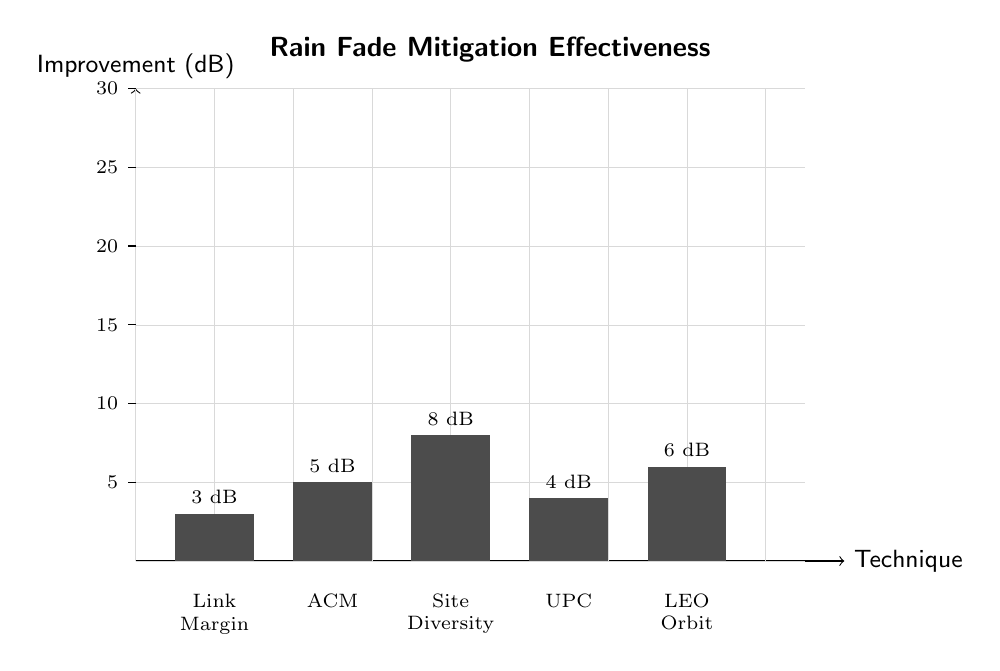
\begin{tikzpicture}[scale=1.0]
% Title
\node[font=\sffamily\bfseries] at (4.5,6.5) {Rain Fade Mitigation Effectiveness};

% Axes
\draw[->] (0,0) -- (9,0) node[right] {\sffamily\small Technique};
\draw[->] (0,0) -- (0,6) node[above] {\sffamily\small Improvement (dB)};

% Grid
\draw[very thin,gray!30] (0,0) grid[step=1] (8.5,6);

% Y-axis ticks
\foreach \y/\label in {1/5,2/10,3/15,4/20,5/25,6/30} {
  \draw (0,\y) -- (-0.1,\y) node[left,font=\scriptsize] {\label};
}

% Bars
\fill[black!70] (0.5,0) rectangle (1.5,0.6); % Link margin
\fill[black!70] (2,0) rectangle (3,1); % ACM
\fill[black!70] (3.5,0) rectangle (4.5,1.6); % Site diversity
\fill[black!70] (5,0) rectangle (6,0.8); % UPC
\fill[black!70] (6.5,0) rectangle (7.5,1.2); % LEO orbit

% Labels
\node[below,font=\scriptsize,align=center,text width=1.5cm] at (1,-0.3) {Link\\Margin};
\node[below,font=\scriptsize,align=center,text width=1.5cm] at (2.5,-0.3) {ACM};
\node[below,font=\scriptsize,align=center,text width=1.5cm] at (4,-0.3) {Site\\Diversity};
\node[below,font=\scriptsize,align=center,text width=1.5cm] at (5.5,-0.3) {UPC};
\node[below,font=\scriptsize,align=center,text width=1.5cm] at (7,-0.3) {LEO\\Orbit};

% Values on top of bars
\node[above,font=\scriptsize] at (1,0.6) {3 dB};
\node[above,font=\scriptsize] at (2.5,1) {5 dB};
\node[above,font=\scriptsize] at (4,1.6) {8 dB};
\node[above,font=\scriptsize] at (5.5,0.8) {4 dB};
\node[above,font=\scriptsize] at (7,1.2) {6 dB};
\end{tikzpicture}
\end{center}

\section{Summary}

\subsection{Key Principles}

\begin{enumerate}
\item \textbf{Frequency Dependence:} Attenuation increases dramatically above 10~GHz
\item \textbf{Quadratic Scaling:} Loss proportional to $R^\alpha$ where $\alpha \approx 1.0$--1.3
\item \textbf{Path Length:} Longer paths through rain accumulate more loss
\item \textbf{Rain $\gg$ Fog:} Rain dominates at microwave/mmWave; fog matters at THz
\end{enumerate}

\subsection{Rain Attenuation by Band}

\textbf{Path:} 6~km slant through rain (satellite, $30°$ elevation)

\textbf{Path}: 6 km slant through rain (satellite,
30\$\^{}\textbackslash circ\$ elevation)

{\def\LTcaptype{} % do not increment counter
\begin{longtable}[]{@{}
  >{\raggedright\arraybackslash}p{(\linewidth - 8\tabcolsep) * \real{0.0759}}
  >{\raggedright\arraybackslash}p{(\linewidth - 8\tabcolsep) * \real{0.1392}}
  >{\raggedright\arraybackslash}p{(\linewidth - 8\tabcolsep) * \real{0.2785}}
  >{\raggedright\arraybackslash}p{(\linewidth - 8\tabcolsep) * \real{0.2658}}
  >{\raggedright\arraybackslash}p{(\linewidth - 8\tabcolsep) * \real{0.2405}}@{}}
\toprule\noalign{}
\begin{minipage}[b]{\linewidth}\raggedright
Band
\end{minipage} & \begin{minipage}[b]{\linewidth}\raggedright
Frequency
\end{minipage} & \begin{minipage}[b]{\linewidth}\raggedright
12 mm/hr (Temperate)
\end{minipage} & \begin{minipage}[b]{\linewidth}\raggedright
42 mm/hr (Tropical)
\end{minipage} & \begin{minipage}[b]{\linewidth}\raggedright
95 mm/hr (Extreme)
\end{minipage} \\
\midrule\noalign{}
\endhead
\bottomrule\noalign{}
\endlastfoot
C & 4 GHz & 0.15 dB & 0.7 dB & 2 dB \\
C & 6 GHz & 0.3 dB & 1.3 dB & 3.5 dB \\
X & 10 GHz & 0.5 dB & 2.5 dB & 7 dB \\
Ku & 12 GHz & \textbf{3 dB} & \textbf{9 dB} & \textbf{25 dB} \\
Ku & 14 GHz & 4 dB & 11 dB & 30 dB \\
Ka & 20 GHz & \textbf{7 dB} & \textbf{22 dB} & \textbf{55 dB} \\
Ka & 30 GHz & 13 dB & 38 dB & 90 dB \\
V & 40 GHz & 22 dB & 60 dB & 140 dB \\
V & 50 GHz & 30 dB & 80 dB & 180 dB \\
\end{longtable}
}

\textbf{Bold:} Typical link budget fades (manageable with standard margins)

\subsection{Design Guidelines}

\begin{center}
\begin{tabular}{@{}llll@{}}
\toprule
Band & Temperate Margin & Tropical Margin & Best Use Case \\
\midrule
C (4--8~GHz) & 1--2~dB & 2--4~dB & Critical services, tropics \\
Ku (12--18~GHz) & 3--5~dB & 8--15~dB & Standard satellite TV/data \\
Ka (20--30~GHz) & 8--12~dB & 15--25~dB & HTS with ACM \\
V (40--75~GHz) & 15--25~dB & Impractical & Research, LEO links \\
\bottomrule
\end{tabular}
\end{center}

\section{Further Reading}

\begin{itemize}
\item \textbf{Free-Space Path Loss (FSPL):} Baseline propagation loss calculation
\item \textbf{Atmospheric Effects (Ionospheric, Tropospheric):} Clear-air propagation phenomena
\item \textbf{Multipath Propagation \& Fading:} Rayleigh/Rician fading (different mechanism)
\item \textbf{Signal-to-Noise Ratio (SNR):} Impact of attenuation on link quality
\item \textbf{QPSK Modulation / LDPC Codes:} ACM adapts these for rain conditions
\item \textbf{Adaptive Modulation \& Coding (AMC):} Dynamic link optimization
\item \textbf{Complete Link Budget Analysis:} End-to-end system design
\item \textbf{Antenna Theory Basics:} Larger antennas provide more gain margin
\end{itemize}

\begin{keyconcept}
\textbf{Key Takeaway:} Rain fade increases dramatically with frequency. C-band is robust but bandwidth-limited. Ka-band and above require sophisticated mitigation (ACM, diversity, large margins) for reliable service, especially in tropical regions. Modern LEO constellations leverage shorter paths for improved Ka-band performance.
\end{keyconcept}
